\documentclass[12pt, letterpaper]{article}
\usepackage[ngerman]{babel}
\usepackage{graphicx}
\usepackage{wrapfig}
\usepackage{titlesec}
\usepackage{geometry}
\usepackage[font=scriptsize]{caption}
\usepackage{blindtext}
\usepackage{hyperref}
\usepackage{tabularx}
\usepackage{subcaption}
\usepackage{verbatim}
\usepackage{fancyvrb}
\hypersetup{
  colorlinks = true,
  linkcolor = black,
  urlcolor = blue,
}

% \captionsetup{justification=raggedright,singlelinecheck=false}
\geometry{
 a4paper,
 total={170mm,257mm},
 left=20mm,
 top=20mm,
 }
%  \titleformat{\section}[display]
%    {\normalfont\bfseries}{}{0pt}{\huge}
  
\usepackage{lipsum}  
\graphicspath{ {./Bilder/} }
\author{Oleksii Baida}
\date{Mai 2024}
\begin{document}
\begin{titlepage}
  
\includegraphics[width = 0.25\pdfpagewidth]{./Bilder/FHDO.jpg}
  \begin{center}
    
    \huge \textbf{\textsf{PA2}} \\
    \vspace{3cm}
    \large \textbf{Oleksii Baida}\\
    \textbf{Matrikelnummer 7210384}\\
    \vspace{3cm}
    \large \textbf{Projektarbeit 2}\\
    \vspace{1cm}
    \large \textbf{Bericht}\\
    \vspace{1cm}
    \today
  \end{center}
\end{titlepage}

\tableofcontents
\pagebreak

\section{Einleitung}

\section{Verbindungstheorie}
\subsection{MQTT}
\subsubsection{MQTT}
\par Das MQTT-Protokoll\footnote[1]{Message Queuing Telemetry Transport} ist ein einfaches, effizientes und leichtgewichtiges Nachrichtenprotokoll, das speziell für den Einsatz in IoT-Systemen entwickelt wurde. Es ermöglicht die Kommunikation von Geräten mit geringer Bandbreite und begrenzten Ressourcen. Das Protokoll basiert auf dem Publish-Subscribe-Modell und erfordert daher eine zentrale Instanz, den Broker. Dies ermöglicht es den Geräten, Nachrichten an einen zentralen MQTT-Broker zu senden und von diesem zu empfangen. Die Nachrichten werden unter Topics veröffentlicht, welche Kanäle darstellen, zu denen sich Subscriber registrieren können. Das Backend für das MQTT-Protokoll kann mit NodeRed realisiert werden. NodeRed bietet ein sehr benutzerfreundliches Interface, um die Nachrichten vom Publisher zu empfangen, zu verarbeiten und an ein Endgerät zu senden, wie zum Beispiel einen Telegram-Bot oder ein Cloud-System.
\par MQTT wird aufgrund seiner Unkompliziertheit oft in Smart-Home-Anwendungen verwendet. Es zeichnet sich durch eine gute Zuverlässigkeit aus, da die Nachrichten immer in einer bestimmten Reihenfolge vermittelt werden. Jede Nachricht wird genau einmal gesendet. Obwohl es keine Garantie für die Zustellung der Nachricht gibt, werden Duplikate vermieden. MQTT ermöglicht das Speichern der letzten Nachricht im Topic, wodurch neue Abonnenten diese Nachricht sofort nach der Registrierung zum Topic erhalten. Aus eigener Erfahrung kann ich bestätigen, dass es bei häufigem Senden der Nachrichten keine Probleme mit der Zustellung gibt. Wenn Nachrichten für eine bestimmte Zeit ausbleiben, sollte überprüft werden, ob die Verbindung unterbrochen ist. MQTT bietet Last-Will-und-Testament-Funktion, was ermöglicht dem Broker eine bestimmte Nachricht bei dem Ausfall der Verbindung zu senden. Diese Nachricht kann bei der Registrierung des Subscribers zum Topic definiert werden und wird im Brocker gespeichert, bis er einen Verbindungsausfall erkennt.
\par Bei der Wahl des Protokolls sollten die Entwickler die folgenden Schlüsselpunkte berücksichtigen:
\begin{itemize}
  \item[\textbullet] \textbf{Data latency} – Wie schnell sollen die Daten übergeben werden? Wie kann man ein Packet vom Startpunkt zum Endpunkt vernünftig übergeben?
  \item[\textbullet] \textbf{Reliability} – Welche Folgen hat Datenverlust im IoT-System? Wie kann das System zuverlässiger werden?
  \item[\textbullet] \textbf{Bandwidth} – Wie groß sind Datenmengen, die transportiert werden sollen?
  \item[\textbullet] \textbf{Transport} – Welches Protokoll ist für den Transport am besten geeignet? Am meisten wird zwischen TCP, UDP und HTTP entschieden.
\end{itemize}

\subsection{UART}
\par Hier wird die UART-Verbindung ESP-Arduino beschrieben
\subsection{WLAN}
\par Hier wird die WLAN-Verbindung ESP-Raspberry beschrieben

\section{Raspberry Pi}
\subsection[Überblick]{Was ist Raspberry Pi?}
\par Für das Projekt verwende ich einen Raspberry Pi 1.0 Modell B+. Raspberry Pi ist ein kompakter und kostengünstiger Einplatinencomputer. Er ist mit einem ARM-Prozessor, 512 MB RAM, USB-Ports, MicroSD-Kartensteckplatz, HDMI- und Ethernet-Anschluss sowie GPIO-Pins ausgestattet. Zusätzlich verfügt der Raspberry Pi über Wi-Fi- und Bluetooth-Funktionalität, die eine kabellose Vernetzung und Datenübertragung ermöglicht. Die Stromversorgung erfolgt über einen Micro-USB-Anschluss. Auf dem Raspberry Pi läuft das Betriebssystem Raspberry Pi OS, das auf Debian 12 "Bookworm" basiert. 
\par In meinem Projekt verwende ich den Raspberry Pi als zentralen Server des Systems sowie den MQTT-Broker. Die Verbindung zwischen dem ESP8266 und dem Raspberry Pi erfolgt über WLAN. Dazu müssen beide Geräte an ein Netzwerk angeschlossen werden. Hierfür gibt es zwei Möglichkeiten: entweder werden die beiden Geräte über ein Heimnetzwerk mit dem Router verbunden, oder das Netzwerk wird vom Raspberry Pi zur Verfügung gestellt. Für mein Projekt habe ich mich für die zweite Variante entschieden. Der Raspberry Pi wird als ein Access Point konfiguriert und über Ethernet mit dem Internet verbunden. Der ESP8266 verbindet sich dann mit dem MQTT-Broker, der auf dem Raspberry Pi gehostet wird. Der Raspberry übernimmt somit die Rolle eines Routers. Dies hat folgende Vorteile:
\begin{itemize}
  \item Das lokale WLAN-Netzwerk kann direkt am Raspberry Pi konfiguriert werden. Das vereinfacht die Verbindung der angeschlossenen Geräten sowie die Überwachung der Datenübertragung.
  \item Die Sicherheit der Verbindung wird dadurch erhöht, dass das lokale WLAN von außen (aus dem Internet) nicht sichtbar ist. Zusätzlich kann auf dem Raspberry Pi eine Firewall für die Internetverbindung eingerichtet werden.
  \item Das gesamte System ist portabler. Wenn das System an einem anderen Ort installiert wird, muss nur die Internetverbindung mit dem Raspberry Pi eingerichtet werden. Das lokale WLAN muss nicht angepasst werden.
\end{itemize}
\par Weiter unten wird die Einstellung des Raspberry Pi beschrieben.

\subsection{Einrichtung als Access Point}
\par Für die Einrichtung des Raspberry Pi als WLAN Access Point wird das Softwarepaket \texttt{hostapd}\footnote[1]{Host Access Point Daemon} verwendet. Mit Hilfe von hostapd können normale Netzwerkkarten in Access Points umgewandelt werden. Für meine Zwecke muss das Interface \texttt{wlan0} als Access Point umgewandelt werden.
\par Zunächst muss das Paket auf dem Raspberry Pi installiert werden. 
\begin{Verbatim}[frame=single]
  sudo apt-get install hostapd
\end{Verbatim}
Für die Konfiguration des Access Points muss die Konfigurationsdatei  erstellt werden. 
\begin{Verbatim}[frame=single]
  sudo nano /etc/hostapd/hostapd.conf

  #Konfigurationsdatei für hostapd
  
  interface=wlan0
  driver=nl80211
  country_code=DE
  ssid=RaspEsp
  hw_mode=g
  channel=6
  wmm_enabled=0
  macaddr_acl=0
  auth_algs=1
  ignore_broadcast_ssid=0
  wpa=2
  wpa_passphrase=mqtt1234
  wpa_key_mgmt=WPA-PSK
  wpa_pairwise=TKIP
  rsn_pairwise=CCMP

  #End
\end{Verbatim}
\par In Bezug auf die Vielzahl an verfügbaren Optionen, die sich für die Konfiguration des hostapd anbieten, habe ich für mein Projekt folgende Einstellungen gewählt: 
\begin{itemize}
  \item[\textbullet] \textbf{interface} --- bezeichnet das Interface, das zu Access Point konfiguriert wird.
  \item[\textbullet] \textbf{driver} --- nl80211 ist der standarte, meistverwendete Driver für \texttt{hostapd}.
  \item[\textbullet] \textbf{country\_code} --- bezeichnet das Land, wo das Netzwerk läuft.
  \item[\textbullet] \textbf{ssid} --- der Name des Netzwerks.
  \item[\textbullet] \textbf{hw\_mode}  --- Operation Mode. 'g' steht für Standard IEEE 802.11g.
  \item[\textbullet] \textbf{channel} --- der verwendete Kanal für die WLAN-Verbindung
  \item[\textbullet] \textbf{wmm\_enabled} --- Wireless Multimedia Extension muss für die WLAN-Verbindung aktiviert sein.
  \item[\textbullet] \textbf{macaddr\_acl} --- Authentifizierung auf Basis des MAC-Protokolls. 0 akzeptiert alle MAC-Adressen, die nicht in Ablehnungsliste sind.
  \item[\textbullet] \textbf{auth\_algs} --- Shared-Key-Authentifizierung
  \item[\textbullet] \textbf{ignore\_broadcast\_ssid} --- Standardeinstellung. Ignoriert Anfragen, die kein vollständiges SSID erhalten.
  \item[\textbullet] \textbf{wpa} --- Wi-Fi Protected Access. Art der Sicherheit des Access Points. Für das Projekt wird WPA 2 verwendet.
  \item[\textbullet] \textbf{wpa\_passphrase} --- das Passwort für den Access Points
  \item[\textbullet] \textbf{wpa\_key\_mgmt, wpa\_pairwise, rsn\_pairwise} --- sind für WPA 2 benötigt.
\end{itemize}
\par Anschließend soll das hostapd automatisch beim Hochfahren starten. Dazu ist es erforderlich, die Einstellungen für den Systemstart anzupassen
\begin{Verbatim}[frame=single]
  sudo nano /etc/default/hostapd

  #Auskommentieren oder neu schreiben
  DAEMON\_CONF="/etc/hostapd/hostapd.conf"
\end{Verbatim}
\par Nun ist der \texttt{hostapd} konfiguriert, aber noch nicht gestartet. Die beiden Befehle starten die \texttt{hostapd}:
\begin{Verbatim}[frame=single]
  sudo systemctl unmask hostapd
  sudo systemctl enable hostapd

  sudo reboot #Neustart des Raspberry Pi
\end{Verbatim}
\par Danach wird ein Neustart des Raspberry Pi empfohlen, um die Änderung anzuwenden. Der Access Point sollte nun mit entsprechendem SSID auf anderen Geräten sichtbar sein, allerdings ist eine Verbindung zu ihm nicht möglich. Um die Verbindung zu ermöglichen, müssen der DNS- sowie der DHCP-Server auf dem Raspberry Pi eingerichtet werden.

\subsection{Einrichtung des DNS- und DHCP-Servers}
\par Der DNS\footnote[2]{Domain Name System}-Server übersetzt Domains in die IP-Adressen. Der DHCP\footnote[3]{Dynamic Host Configuration Protocol}-Server weist die IP-Adressen den verbundenen Geräten zu. Für die reibungslose Verbindung und Kommunikation müssen beide Server auf dem Raspberry PI eingerichtet werden.
\par Für die Konfiguration des DNS-Servers sowie des DHCP-Servers wird das Softwarepaket \texttt{dnsmasq} verwendet. Das Paket ermöglicht eine einfache und schnelle Konfiguration der beiden Server auf Linux-basierten Systemen.
\par In der Konfigurationsdatei sind eine Vielzahl an die Optionen für die Einstellung des DNS-Servers vorgegeben, wobei lediglich ein Teil davon für die Bearbeitung relevant ist.
\begin{Verbatim}[frame=single]
  sudo nano /etc/dnsmasq.conf

  #Konfigurationsdatei für DNS-Server
  #Auskommentieren oder neu schreiben
  interface=wlan0
  bind-dynamic
  domain-needed
  bogus-priv
  dhcp-range=192.168.1.100,192.68.1.110,255.255.255.0,12h

  #End
\end{Verbatim}
\begin{itemize}
  \item[\textbullet] \textbf{interface} --- definiert Interface, an welchem der DNS-Server fungiert.
  \item[\textbullet] \textbf{bin-dynamic} --- erlaubt die Verbindung nur mir exsistierenden Inrefaces.
  \item[\textbullet] \textbf{domain-needed} --- ignoriert DNS-Anfragen ohne Domänennamen. 
  \item[\textbullet] \textbf{bogus-priv} --- die DNS-Anfragen aus lokalem Netzwerk werden nicht an Haupt-DNS-Server weitegeleitet.
  \item[\textbullet] \textbf{dhcp-range} --- gibt den Bereich der IP-Adressen für DHCP-Server an.
\end{itemize}
\par Anschließend muss der DHCP-Server eingerichtet werden.
\begin{Verbatim}
  sudo nano /etc/dhcpcd.conf

  #Konfigurationsdatei für DHCP-Server
  nohook wpa_supplicant
  interface=wlan0
  static ip_address=192.168.1.10/24
  static routers=192.168.1.1
\end{Verbatim}
\par Entsprechend den oben beschriebenen Einstellungen werden die IP-Adressen von 192.168.1.100 bis 192.168.1.110 durch den DHCP-Server verteilt und laufen nach 12 Stunden automatisch ab. Für den Host (Raspberry Pi) ist die IP-Adresse 192.168.1.10 reserviert. Default-Gateway hat die IP-Adresse 192.168.1.1 
\subsection{MQTT-Broker}
\par Der MQTT Broker ermöglicht die Kommunikation zwischen den MQTT-Geräten. Der Broker empfängt Nachrichten von sogenannten "Publishern" und leitet sie an "Subscriber" weiter. Die Subscriber müssen sich für bestimmte Themen (Topics) registrieren.
\par In meinem System läuft der MQTT-Broker auf dem Raspberry Pi. Für die Einrichtung des Brokers wird das Softwarepaket \texttt{mosquitto}\footnote[99]{https://mosquitto.org/} verwendet. Mosquitto erlaubt schnelle und einfache Einstellung und Verwaltung von MQTT-Broker. 
\par 
\begin{enumerate}
  \item Installation:
\begin{Verbatim}[frame=single]
  sudo apt install mosquitto mosquitto-clients
\end{Verbatim}
\item Autostart einschalten:
\begin{Verbatim}[frame=single]
  sudo systemctl enable mosquitto
  sudo systemctl start mosquitto
\end{Verbatim}
\item Konfiguration:
\begin{Verbatim}[frame=single]
  sudo nano /etc/mosquitto/mosquitto.conf

  listener 1883
  allow_anonymous true
\end{Verbatim}
\par allow\_anonymous für die Ersteinrichtung und zu Testzwecken einschalten. Die Konfiguration der Benutzer erfolgt weiterhin im Text LINK.
\item Konfigurationsdatei speichern \texttt{Strg+O} und schließen \texttt{Strg+X} und Mosquitto neu starten 
\begin{Verbatim}[frame=single]
  sudo systemctl restart mosquitto
\end{Verbatim}
  \item Testen. Ein Subscriber für Topic registrieren: 
\begin{Verbatim}[frame=single]
  mosquitto_sub -h localhost -t <DEIN_TOPIC>
\end{Verbatim}
\par Neues Fenster öffnen \texttt{Strg+T} und über einen Publisher eine Nachricht in das Topic senden.
\begin{Verbatim}[frame=single]
  mosquitto_pub -h localhost -t <DEIN_TOPIC> -m "MEINE 1. MQTT-NACHRICHT"
\end{Verbatim}
\par Nach dem Parameter -t (Topic) keine Klammern setzen. Nach dem Parameter -m (Message) den Text der Nachricht in Klammern setzen.
\end{enumerate}
\section{ESP8266}
\subsection[Überblick]{Was ist ESP8266?}
\par Das ESP8266 ist ein kleines, günstiges WLAN-Modul. Es wurde von Espressif Systems entwickelt. Das Modul ermöglicht die kabellose Verbindung von Mikrocontrollern mit dem Internet. In meinem Projekt verwende ich das ESP8266, um den Arduino drahtlos mit dem Raspberry PI zu verbinden.
\par Der ESP8266 basiert auf einem 32-Bit-Prozessor und hat einen Systemtakt von 80 MHz bis 160 MHz. Das Modul verfügt über 64 kB RAM als Befehlsspeicher und 96 kB RAM als Datenspeicher. Das ESP8266 besitzt keinen internen Flash-Speicher für die Firware. Ansonsten wird die Firmware in einem externen Flash-Speicher abgelegt und wird blockweise in den RAM-Speicher geladen. Je nach Modell verfügt das ESP8266 über verschiedene Schnittstellen wie I/O-Ports und I2C. Ich verwende das Modell mit WLAN und UART \footnote[1]{Universal Asynchronous Receiver-Transmitter}. Über den UART-Port wird der Programmcode in das ESP8266 geladen. Das Modul muss mit einer Spannung von 5 V versorgt werden.
\par Der ESP8266 ist mit vielen Programmiersprachen kompatibel. Für die Programmierung des Moduls verwende ich Visual Studio Code mit der PlatformIO Erweiterung. 
\subsection[Arduino-ESP8266]{Verbindung von Arduino und ESP8266}
\par Die Verbindung zwischen Arduino und ESP8266 kann auf unterschiedliche Weise hergestellt werden. Im Rahmen meines Projekts erfolgt die Verbindung über eine serielle UART-Schnittstelle.
\par Der Arduino verfügt über RX- und TX-Pins (Pin 0 und 1) für die serielle Kommunikation. Der RX-Pin des Arduino muss mit dem TX-Pin auf dem ESP8266 verbunden werden und der TX-Pin umgekehrt.In der Folge können die Daten des Arduino über die Funktion Serial.print() an das Modul ESP8266 über die serielle Schnittstelle übermittelt werden. Dabei ist zu berücksichtigen, dass bei einer Verbindung des Arduino mit einem Rechner über den USB-Port der Arduino den USB-Port als serielle Schnittstelle definiert. Infolgedessen werden keine Daten über die TX- bzw. RX-Ports übergeben. Daher ist eine Versorgung des Arduino mittels eines Netzteiles mit 5 V erforderlich.
\par Aufgrund der Weiterleitung der Daten vom Arduino über die MQTT-Verbindung ist eine entsprechende Berücksichtigung der jeweiligen Formatierung erforderlich. Der Arduino übermittelt die Befehle mit dem Format \"topic:message\". Dies erleichtert dem ESP8266 die Verarbeitung der empfangenen Nachricht sowie deren Weiterleitung mit dem entsprechenden Topic. Auf der Abbildung \ref{abb:readserial} ist der Programmcode für die Verarbeitung der Daten von Arduino zu sehen. 
\begin{figure}[h]
  \begin{subfigure}[b]{0.45\textwidth}
    \centering
    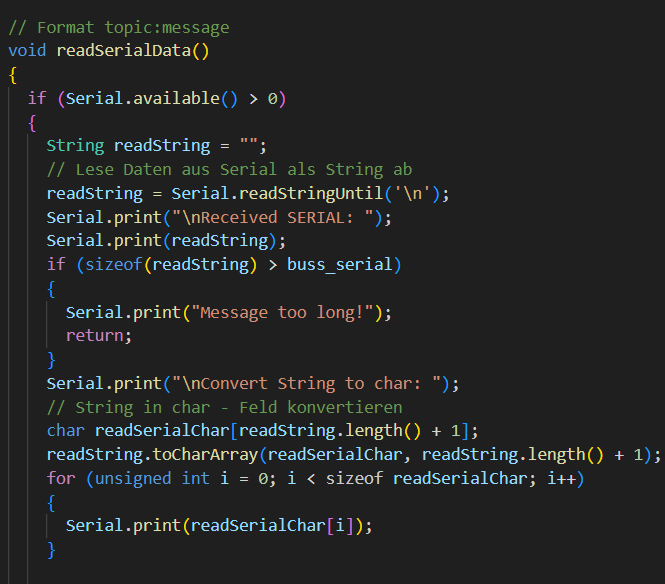
\includegraphics[width=\textwidth]{readSerial2.png}
  \end{subfigure}
  % \hspace{0.05\textwidth}
  \begin{subfigure}[b]{0.45\textwidth}
    \centering
    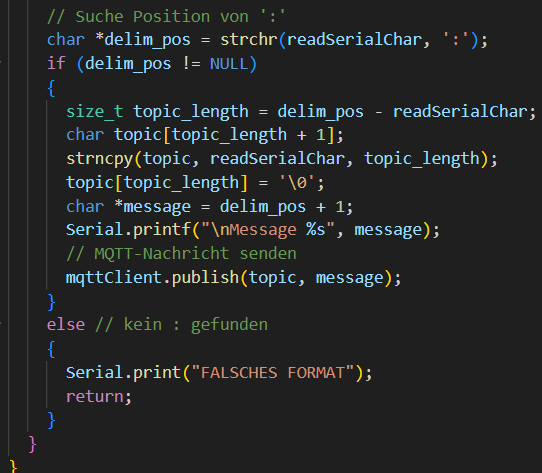
\includegraphics[width=\textwidth]{readSerial1.png}
  \end{subfigure}
  \caption{Verarbeitung der Daten vom Arduino}
  \label{abb:readserial}
\end{figure}
\subsection[ESP8266-Raspberry Pi]{ESP8266 als Schnittstelle für die MQTT-Verbindung}
\par In meinem Projekt verwende ich den ESP8266 für die Erstellung der MQTT-Verbindung zwischen Arduino und Raspberry Pi. Wie oben beschrieben, wird der Raspberry Pi als MQTT-Broker und WLAN-Access-Point eingerichtet. Der ESP8266 muss sich mit dem Zuganspunkt von Raspberry Pi verbinden und eine MQTT-Verbindung zu dem Broker erstellen. Außerdem muss der ESP8266 die Daten von Arduino erhalten.
\subsubsection{Verbindung mit WLAN}
\par Zunächst ist eine Verbindung des ESP8266 mit dem vom Raspberry Pi bereitgestellten WLAN erforderlich. Für diesen Zweck wird die Bibliothek \texttt{ESP8266WIFI.h} verwendet. Es muss ein Objekt \texttt{WifiClient} und zwei konstanten Variablen \texttt{WIFI\_SSID} und \texttt{WIFI\_PASSWORD} erstellt werden. In der Konstante \texttt{WIFI\_SSID} wird der Name des WLAN-Netzwerks gespeichert und in der Konstante \texttt{WIFI\_PASSWORD} wird das Passwort gespeichert.
\par Die Verbindungsroutine ist in der Funktion \texttt{connect\_wifi()} (Abbildung \ref{abb:espwifi}) zu sehen. Diese Funktion wird beim Start des Moduls in der \texttt{setup()}-Funktion aufgerufen.
\begin{figure}[h]
  \centering
  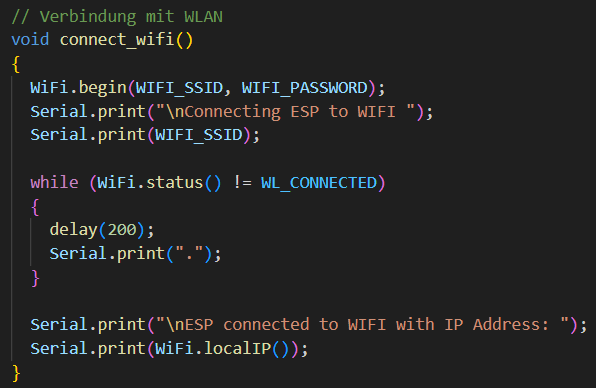
\includegraphics[scale = 1]{connect_wifi.png}
  \caption{ESP8266 connect\_wifi()}
  \label{abb:espwifi}
\end{figure}
\par Das ESP8266 versucht jede 200 Milisekunden sich mit dem WLAN zu verbinden. Die Serial-Ausgaben in der Konsole sind nur für die Testzwecken benötigt. 
\subsubsection{Verbindung mit dem MQTT-Broker}
\par Für die Verbindung des ESP8266 mit dem MQTT-Broker wird eine Bibliothek \texttt{PubSubClient.h} verwendet. Es ist erforderlich, dass der MQTT-Broker mit dem gleichen Netzwerk wie der ESP8266 verbunden ist. In meinem System läuft der Broker auf dem Raspberry Pi und das WLAN wurde auch vom Raspberry Pi zur Verfügung gestellt. So befinden sich die beiden Module in einem Netzwerk. 
\par Im Programmcode am ESP8266 muss ein Objekt \texttt{PubSubClient} erstellt werden. Als Parameter wurde den \texttt{WifiClient} übergeben. In der konstanten Variable \texttt{MQTT\_BROKER\_ADRRESS} ist die IP-Adresse des Brokers und in der Variable \texttt{MQTT\_PORT} ist die Portnummer gespeichert. Die Verbindungsroutine ist in die Funktion \texttt{connect\_mqtt()} (Abbildung \ref{abb:connect_mqtt}) eingepackt. Diese Funktion wird beim Start von ESP8266 in der \texttt{setup()}-Funktion aufgerufen.
\begin{figure}[h]
  \centering
  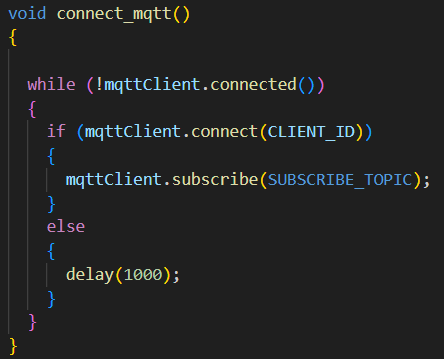
\includegraphics[scale=1]{connect_mqtt.png}
  \caption{ESP8266 connect\_mqtt()}
  \label{abb:connect_mqtt}
\end{figure}
\par Nach erfolgreicher Erstellung der Verbindung mit dem MQTT-Broker muss das ESP8266 das Topic \texttt{UBSCRIBE\_TOPIC} abonnieren, um die Befehle von dem Broker zu erhalten. Das ermöglicht beideseitige Kommunikation zwischen ESP8266 und MQTT-Broker.
\par Sobald das ESP8266 die Daten von dem Arduino empfängt, wird die MQTT-Nachricht an den MQTT-Broker mit dem Befehl \texttt{mqttClient.publish(topic, message)} versandt (Abbildung \ref{abb:readserial}).
\par Die Verarbeitung der empfangenen Nachricht erfolgt in der \texttt{callback}-Funktion (Abbildung \ref{abb:callback}). Für die Testzwecken wird die Nachricht sofort in das Topic \texttt{PUBLISH\_TOPIC} gesendet.

\begin{figure}[h]
  \centering
  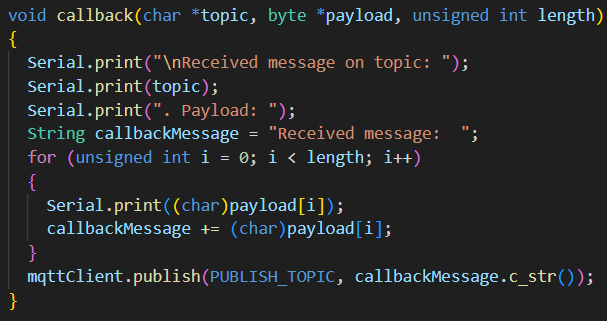
\includegraphics{callback.png}
  \caption{ESP8266 callback()}
  \label{abb:callback}
\end{figure}

\newpage
\listoffigures
\end{document}